% Created 2019-11-11 Mon 15:09
% Intended LaTeX compiler: pdflatex
\documentclass[11pt]{article}
\usepackage[utf8]{inputenc}
\usepackage[T1]{fontenc}
\usepackage{graphicx}
\usepackage{grffile}
\usepackage{longtable}
\usepackage{wrapfig}
\usepackage{rotating}
\usepackage[normalem]{ulem}
\usepackage{amsmath}
\usepackage{textcomp}
\usepackage{amssymb}
\usepackage{capt-of}
\usepackage{hyperref}
\author{Nick Merrill}
\date{\textit{[2019-11-11 Mon]}}
\title{III: What have we learned?}
\hypersetup{
 pdfauthor={Nick Merrill},
 pdftitle={III: What have we learned?},
 pdfkeywords={},
 pdfsubject={},
 pdfcreator={Emacs 25.2.2 (Org mode 9.1.14)}, 
 pdflang={English}}
\begin{document}

\maketitle
We are using a fragmented (ha ha) version of the Network Interference metric for
now, where we look at \textbf{only} website blocking events. We're running up against
the usual troubles with big data, and I certainly expect to compute the full
metric soon, but don't want to put undue pressure on my data discovery student
as she figures things out. Our findings may change a bit as we compute the data,
but my guess is that the major "so what" will remain. As such, I am labeling
these findings ``initial.'' They are no longer ``preliminary,'' but they're not
``final,'' either.

\section{Our main findings}
\label{sec:org814cd39}

\subsection{The Internet is far from bi-polar}
\label{sec:orgd229b3e}

It's tempting to imagine a bi-polar Internet, with China on one, ``non-free''
side, and the West on the other. In this model, it would be tempting to place,
for example, Bahrain on the China ``side.'' Germany might sit on the ``US
side.''

\begin{center}
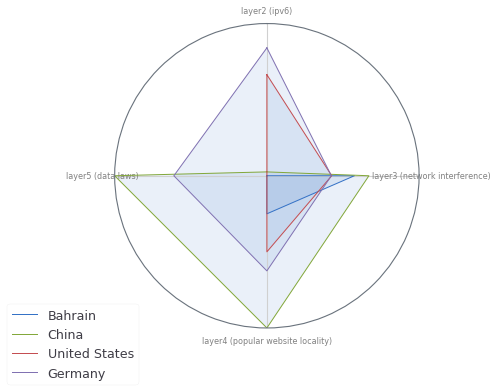
\includegraphics[width=.9\linewidth]{./figures/us-cn-bh-de.png}
\end{center}

Our metrics reveal a much more complex picture. In fact, all four countries
mentioned here have much different profiles to one another.

\subsection{``Blocks'' are often self-similar}
\label{sec:org2862232}

In spite of these surprises, our metrics allow "profiles" of similar to emerge
naturally. Five eyes, Belt and Road, and even regions such as the Caribbean all
show patterns that are similar to one another. Doing so allows us

\begin{center}
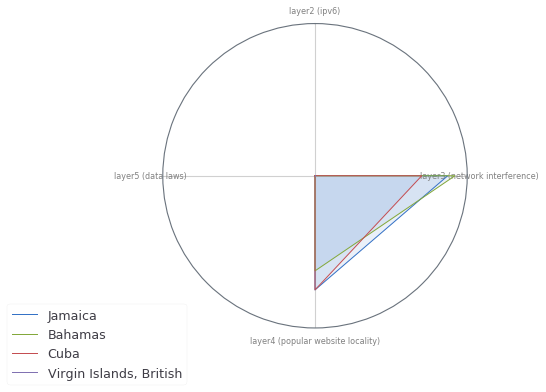
\includegraphics[width=.9\linewidth]{./figures/carribbean.png}
\end{center}
Nevertheless, even within similar blocks, there are important differences to
tease out: IPv6 adoption, content layer differences, and network interference
all vary within otherwise "similar" countries, revealing unexpected differences.
For example, the United States has \uline{XXXXXXXXXXXXXXX} than its Five Eyes allies.

\begin{center}
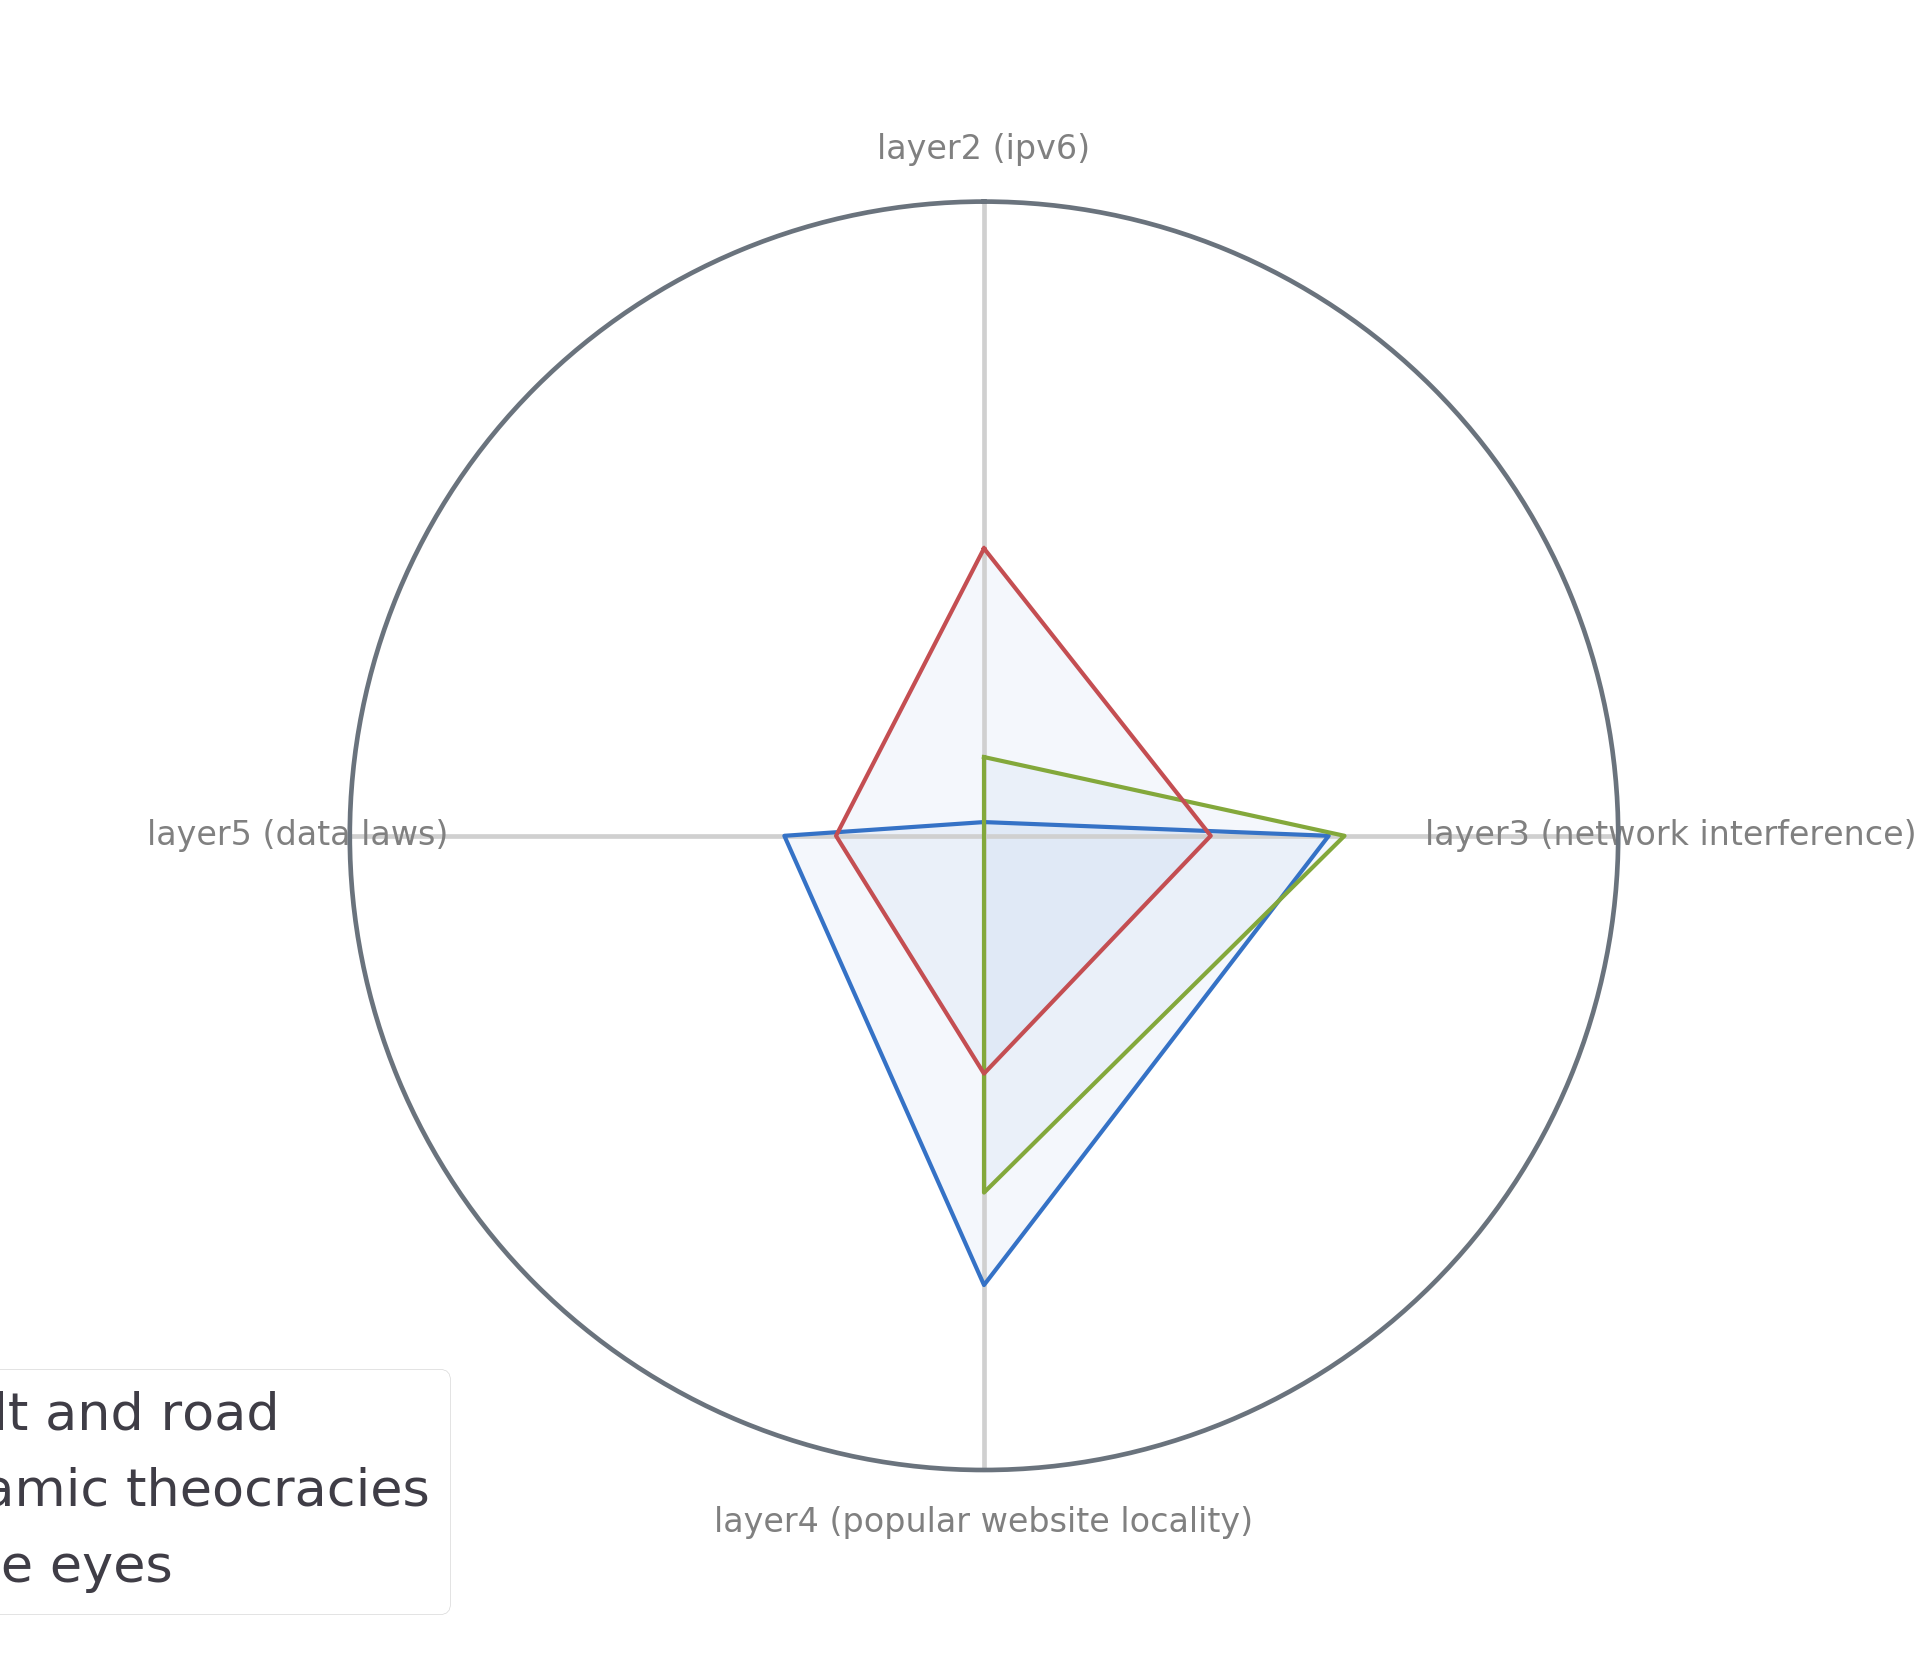
\includegraphics[width=.9\linewidth]{./figures/three-bloc.png}
\end{center}

\subsection{Countries you would expect to be similar can be different in some ways}
\label{sec:org850ad25}
\subsection{Countries you would expect to be different are similar in some ways}
\label{sec:org6835238}
\section{{\bfseries\sffamily TODO} So what?}
\label{sec:org166fe69}
\subsection{{\bfseries\sffamily TODO} What we can do with these findings?}
\label{sec:orga88ef8b}
\subsubsection{Guide policy smooth transitions between markets}
\label{sec:org85c5804}
\begin{enumerate}
\item We can see how countries "stand out from their pack" in particular dimensions
\label{sec:orgd84deda}
like US from 5-eyes
\item How to get from A to B
\label{sec:org63cf1c1}
\end{enumerate}

\subsection{What's next?}
\label{sec:org93b59f4}

are countries interoperable \textbf{with each other}?
for example, right now we look at how smilar content layer is to global,
 but what about argentina's content layer compared to chile's

this is
the \emph{real} ""clusters of internets" question

just calling them out may help them go away
in any case, these clusters could become a key strategic planning tool
 for shifting between markets
 or for crafting policy

\section{{\bfseries\sffamily TODO} Reflections}
\label{sec:orgb699a0a}
\subsection{Am I convinced?}
\label{sec:org0e894b6}

Currently, it's a little difficult to interpret these data outside of their
specific meeting. For example, to me, IPv6 is a more immediate proxy of a
country's "development" (another ambiguous term) than it is a proxy of
"fragmentation."

Of all of the metrics, website locality convinces me the most. It's a measure of
actual user behavior. I am sure network interference matters (and may matter
more if we split it down by interference type), but ultimately, the experience
of e.g., censorship may more acutely felt in the context of website locality (as
is the case with China).

In general, behavioral measures may appear more at the content layer. I'm not
sure that's a bad thing. The content layer shows us what people are, in
practice, doing. Yes, maybe laws that restrict data flows matter, but can we
observe that with actual behavior?

\subsection{{\bfseries\sffamily TODO} What's in a name?}
\label{sec:orgb37c73d}
Really either interoperability \textbf{or} an index right now
more like internet character profiles

we also assume that index is going to be the one thing that sells
maybe, maybe not\ldots{} maybe these indices are also appropriate.
\subsection{{\bfseries\sffamily TODO} Future work}
\label{sec:org4e1fc05}
\subsubsection{Expanding metrics per layer}
\label{sec:orge3cc0c5}

In layer 4, we may be interested in DNS consistency as one measure of
Internet-level fragmentation. DNS consistency has a clear relationship to the
experience of browsing the Internet: what websites \textbf{can} you visit? It would be
worth researching possible sources for this data.

In general, in the future, it's worth thinking about how we would deal with
multiple metrics per layer. They don't fit neatly into our radar graph any more,
and we may have to do some averaging per-layer to compute a composite metric.
There's some art to this, I figure, and we should be mindful of that as we
expand horizontally within TCP/IP layers.
\subsubsection{UI wishlist}
\label{sec:org1d74458}

It would also be great to view metrics in greater detail on rollover. We
certainly want our APIs to support that.
\end{document}
